\section{Experiments}
\begin{figure*}[t]
\subfigure[Implements of Restart Policy with $threshold$ settled as $128$] { \label{fig:a} 
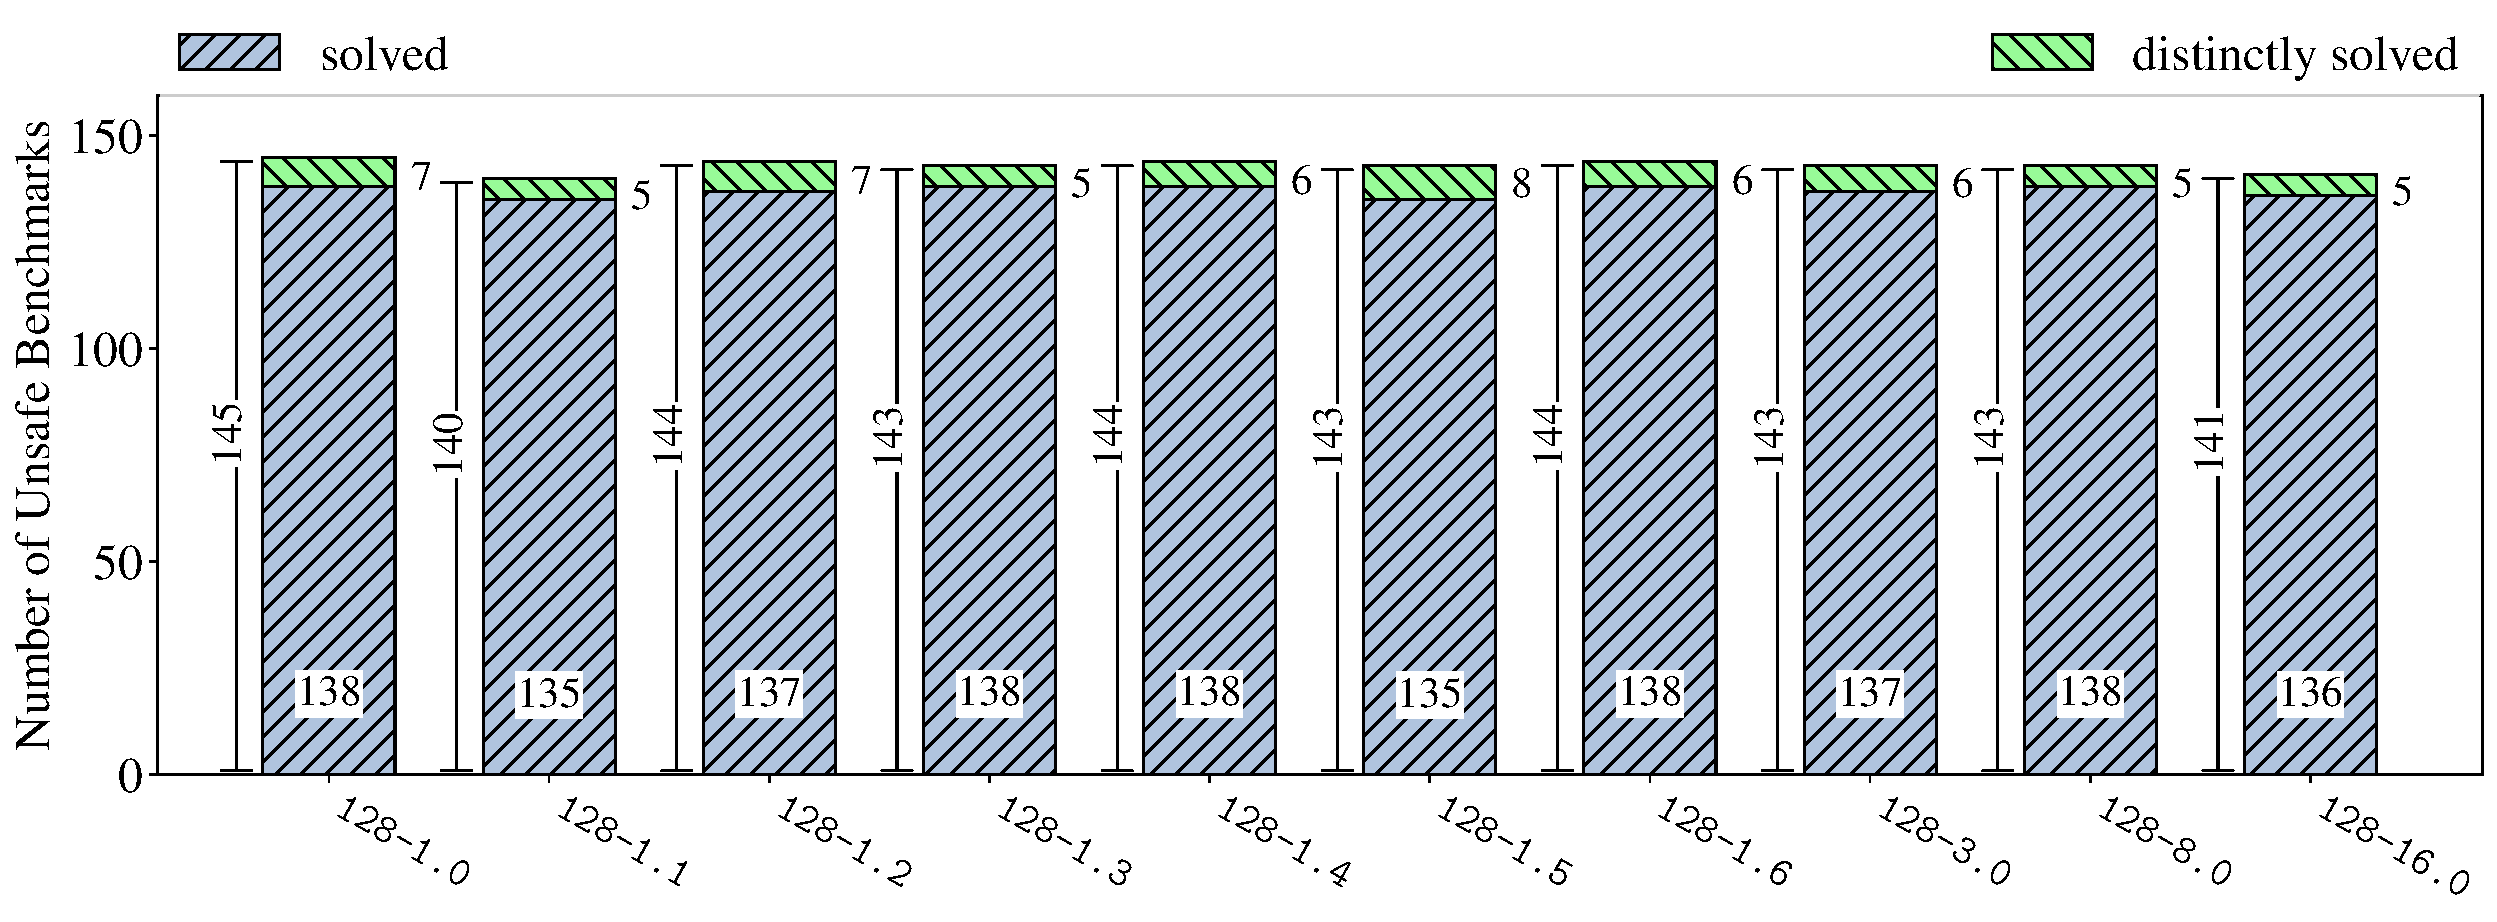
\includegraphics[width=0.98\linewidth]{images/128.pdf} \label{fig:car:128}
}
\subfigure[Implements of Restart Policy with $gr$ settled as $1.2$] { \label{fig:b} 
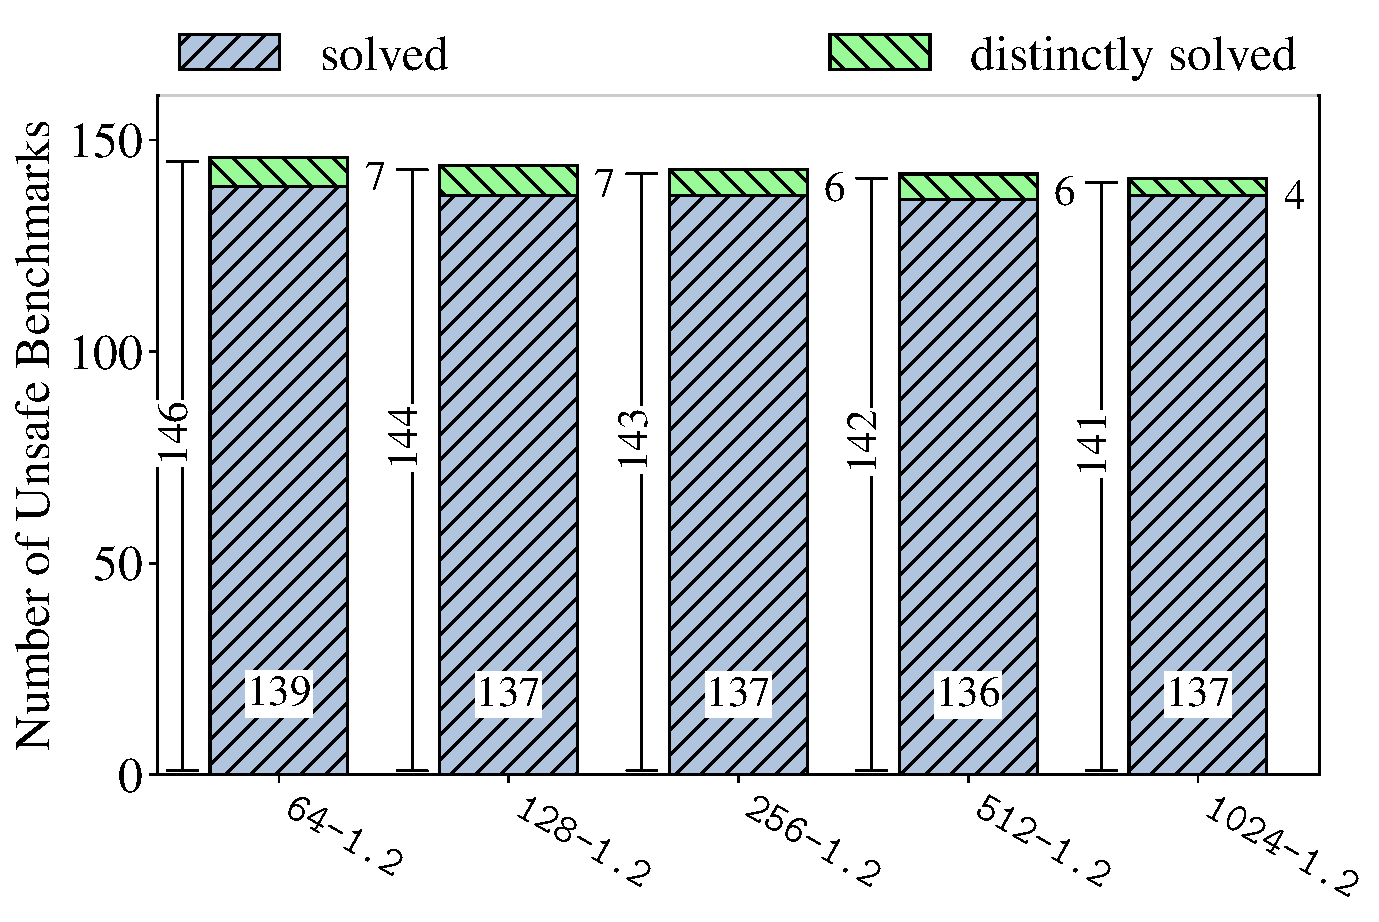
\includegraphics[width=0.49\linewidth]{images/1.2.pdf} \label{fig:car:1.2}
}
\subfigure[CAR vs. BMC] { \label{fig:c} 
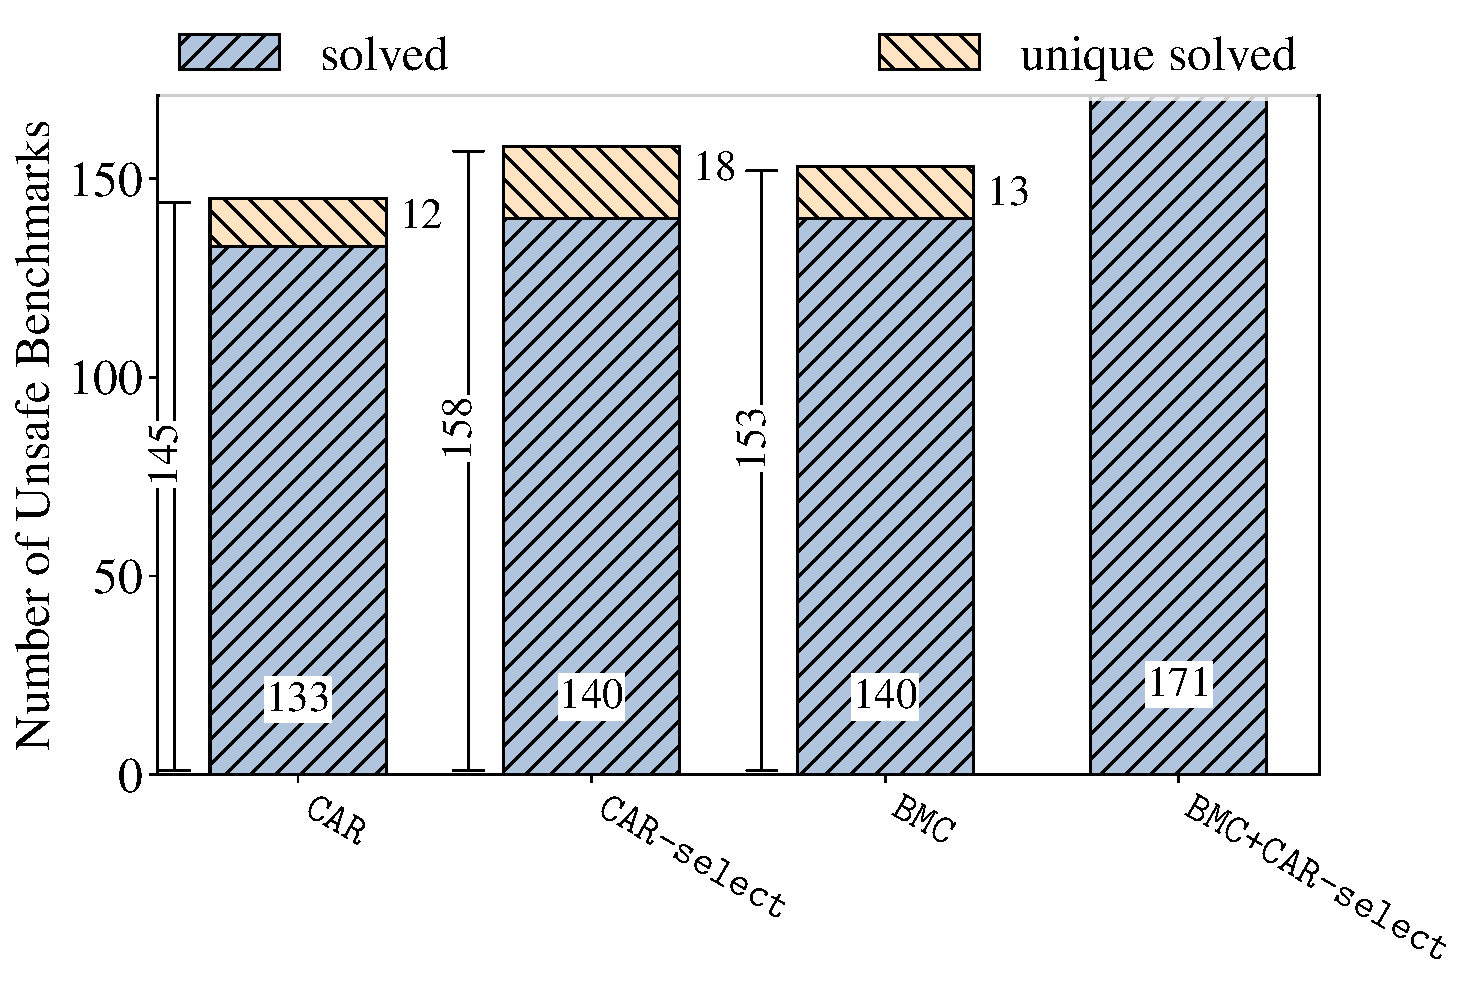
\includegraphics[width=0.49\linewidth]{images/car-bmc.pdf} \label{fig:compare}
}
\caption{Number of unsafe benchmarks solved by CAR after applying the restart policy. The category ``distinctly solved'' benchmarks are solved by CAR with the corresponding restart policy but not by the original CAR. The ``solved'' benchmarks solved by CAR with and without the restart policy. X-axis 128-1.0 means $threshold=128$, $gr=1.0$ and the same applies to others.}\label{fig:car}
\end{figure*}
\subsection{Experimental Setup}
We implement the restart policy to the SimpleCAR model checker \cite{simplecar}. As mentioned before, the restart frequency has a significant influence on the effectiveness of the restart policy. In our conjecture, the frequent restarts in CAR may not preserve the advantages already achieved, while a low frequency of the algorithm cannot help solve new instances. In our proposed algorithm, two parameters $threshold$ and $gr$ are introduced to determine the restart frequency in a dynamic way. We evaluate different combinations of these two parameters. We assign a relatively small value to $threshold$ and assign $gr$ a value equal to or greater than 1 to $gr$, i.e., $threshold = 128, gr = 1.2$, aiming to avoid the disadvantage of frequent restarts by gradually increasing the threshold after each restart. 

We compare our results to those from the original CAR implemented in SimpleCAR, as well as from BMC that is integrated in ABC tool \cite{BM10}, which is a prestigious model checker in the community and won the hardware model checking competition many times. Notably, there are kinds of BMC implementations in ABC, and we select the \emph{bmc2} which has the better performance based on previous evaluations \cite{LDPRV18}. Both SimpleCAR and ABC use the Minisat SAT solver \cite{minisat,ES04} as the computation engine for model checking. 

All the experiments are performed on a cluster consisting of 2304 processor cores in 192 nodes running REDHat 6.0 with a 2.83GHz CPU and 48GB of memory (RAM). In the experiments, the time limit is set to be one hour and the memory-use is 8 GB, for each instance.
We evaluate all algorithms against 749 industrial benchmarks from the single safety property track (SINGLE) of the HWMCC in 2015 \cite{hwmcc15} and 2017 \cite{hwmcc17}. Each instance in the benchmark is an aiger model, which formalizes the And-Invertor Graph \cite{aiger} of a circuit together with the safety property to be verified. 

This paper focuses on unsafe checking, under which a counterexample can be output to help identify the property violation. We use the aigsim tool from the Aiger package \cite{aigertools} to check whether the produced counterexamples are correct. We report that all the counterexamples generated from all checkers pass the test from aigsim.

\subsection{Results}

\subsubsection{Comparison to original CAR}
In the experiments, the original CAR is able to solve 145 unsafe instances without counterexamples.
To evaluate the performance of the restart policy on CAR from this paper, we first fix $threshold$ to be $128$ and make the growth rate $gr$ vary from 1.0 to 16.0. The number of solved and \emph{distinctively solved} (The meaning see the figure.) instances with the corresponding parameters are shown in Fig. \ref{fig:car:128}. From the figure, the restart policy effectively expands the algorithm's diversity by finding considerable new counterexamples with different configurations. In particular, the restart strategy has better results when $gr$ are set to be in $1 < gr < 2$, which are able to gain the most new instances (7 or 8). 


We then vary $threshold$ from 64 to 1024 by fixing $gr$ to be 1.0, 1.2 and 1.5 respectively. The results of setting $gr=1.2$ are shown in 
Fig. \ref{fig:car:1.2}. Observing the results from Fig. \ref{fig:car:1.2}, the restart policy performs the best when the value of $threshold$ is around 128, under which not only more ``distinctly solved'', but also several unique instances are detected. For example, ``oski15a08b15s'' can only be found by ``64-1.2'', ``6s351rb15'' can only be solved by ``128-1.2'' and ``oc8051topo08'' can only be solved by ``128-1.5''. Probably, some instances are sensitive to a particular combo of parameters, which determines the frequency of restart policy. Setting $threshold$ to the value 1024 seems to be too large for a one-hour experiment to make the restart strategy work. 

It should be highlighted that, although IC3/PDR can also perform differently by varying the paremeters to generate the inductive clauses \cite{GR16}, it help more to prove safe instances. Meanwhile, applying the restart policy to CAR results in a better performance on solving unsafe instances that can produce the counterexamples. 

\subsubsection{Comparison to original CAR and BMC }
As shown in Fig. \ref{fig:compare}, the BMC implementation in ABC solve 153 unsafe instances. We combined the results of five experiments(``64-1.2'', ``128-1.2'', ``128-1.5'', ``128-3.0'' and ``256-1.2'')and CAR, noted as ``CAR-select''. Observing ``'CAR-select'', the restart policy helps CAR find 13 more counterexamples (from 145 to 158) and 6 more ``unique solved''(from 12 to 18) that can only solved by CAR. Also, ``CAR-select'' solves 158 instances in total, which outperforms BMC (the amount is 153) and gains 18 instances that can not be found by BMC. The virtual combination of ``CAR-select'' and BMC solves 171 instances, which affirms that the restart policy plays a non-negligible role as a part of the portfolio for hardware model checking.
